
\chapter{Analysis and planning}

\epigraph{As I see it, criticism is the prime \emph{duty} of the
  scientist and of anyone who wants to advance knowledge. Seeing new
  problems and having new ideas, on the other hand, are \emph{not}
  one's duty: originality is, rather, a gift of the gods.}{
  1982 Preface to \emph{Quantum theory and the schism in physics}\\
  \textsc{Karl Popper}}

\section{Requirement modelling}
\label{sec:requirements}

\index{requirement (modelling)}In the following section we discuss the
requirements that we want to impose on our sound synthesis
framework. Note that functional requirements are hard to express for
an API, but a vague description of the desired qualities and features
is still possible and that will guide our development process.

Quite often, we will focus on the final feature that should be
implementable through the framework. Also, note that the framework
already had many features at the beginning of the project, some of
which we will discuss in section \ref{sec:status}. We will try to
avoid describing the requirements related to those ready facilities in
this section, as the only purpose of the requirement modelling is to
aid the actual development of this thesis project. Still, some already
satisfied requirements might be made explicit when some other related
requirement follows, or because of their relevance to the user, or
just for the global consistency of the text.

As we suggested in our objective \ref{obj:artquimia}, these
requirements have been elicited with the assistance of the
ArtQuimia\index{ArtQuimia} Music Production School in order to ensure
the suitability of the software for a productive usage.

\subsection{Functional requirements}

\subsubsection{Basic audio support}

\begin{requirement}
  \label{req:iter1-begin}
  The library must provide data-structures and basic algorithms for
  manipulating audio signals.
\end{requirement}

\begin{requirement}
  The library must provide means to output and input audio data to and
  from files in various formats, including, at least: Microsoft WAV,
  Apple AU and OGG Vorbis.\index{WAV (format)}\index{AU
    (format)}\index{OGG (format)}
\end{requirement}

\begin{requirement}
  \label{req:soundsys}
  \label{req:iter1-end}
  The library must provide means to output and input audio data to and
  from sound-card devices in an asynchronous real-time fashion,
  supporting, at least, the following audio systems:
  ALSA\footnote{Advanced Linux Sound Architecture:
    \url{http://www.alsa-project.org/}}\index{ALSA}, OSS\footnote{Open
    Sound System: \url{http://www.opensound.com/}}\index{OSS},
  Jack\footnote{\url{http://jackaudio.org/}}\index{Jackd}.
\end{requirement}

\subsubsection{Node graph support}

\begin{requirement}
  \label{req:iter2-begin}
  The library must include means for producing the audio as the result
  of executing a dataflow-graph.\index{graph}
\end{requirement}

\begin{requirement}
  The library user must be able to define his own processing
  nodes.\index{node (processing)}
\end{requirement}

\begin{requirement}
  \label{req:porttype}
  Each node should have an arbitrary number of named signal and
  control input and output ports. The difference between signal and
  control ports are that the later are sampled at much less
  frequency.\index{control}\index{port}
\end{requirement}

\begin{requirement}
  Both signal and control ports should be able to process information
  in arbitrary datatypes. Signal ports may have practical limitations
  as for the real-time constraints is concerned.\index{real-time
    constraints}
\end{requirement}

\begin{mynote}[Realtime constraints] \label{note:realtime} All the
  processing done inside the nodes should satisfy soft real-time
  constraints. This is so because in order to produce sound with low
  latency (see requirement \ref{req:latency}) the sound processing
  should be done in blocks (buffers) as small as possible that are
  delivered to the sound-card as soon as possible. If the deadline is
  not met, a disturbing ``click'' sound will be heard because of the
  jump to zero assumed by the sound-card during the period that it did
  not have any audio to output. For example, for a 44100 Hz sampling
  rate and a 128 frames block size, it should take less than $$\frac{1
    s}{44100\ frames}\cdot128\frac{frames}{block}=2.90
  \frac{ms}{block}$$ to process and deliver an audio data
  block.\index{sample rate}

  In practice, this means that the processing algorithms should take
  an amount of time proportional to the amount of data to process ---
  i.e. they are $O(n)$. This in turn disallows writing and reading
  files and most operations that cause non deterministic hardware
  operations or force context switching (mutexes might be unavoidable
  but should be used scarcely). Also, allocation of memory on the heap
  should be avoided because it has a non-predictable and potentially
  non-linear time consumption. Of course, the framework should provide
  hooks to do those forbidden operations outside the audio processing
  thread, but we consider that a design issue that should be addressed
  later.
\end{mynote}

\begin{requirement}\label{req:port-one-to-many}
  Each output port must be connectable to an arbitrary number of input
  ports. Each input port must be connectable to one output port.
\end{requirement}

\begin{requirement}
Ports may be defined statically --- i.e. at compile time --- or
dynamically --- i.e. at runtime.
\end{requirement}

\begin{requirement}
The system must allow the hierarchical composition of nodes, with
special \emph{input} and \emph{output} nodes that are exposed as ports
in the parent level.\index{hierarchy, node}
\end{requirement}

\begin{requirement}
\label{req:iter2-end}\label{req:polyphony}
Nodes can be either monophonic or polyphonic. A polyphonic node,
internally, has several copies of its processing state, called
\emph{voices}, that are dispatched accordingly trough trigger signals.
\index{polyphony}\index{voice (polyphony)}
\end{requirement}

\begin{mynote}[On the scope of polyphony]
We will avoid specifying here details on how polyphony works that are
still quite important as a \emph{usability} concern. For example,
should monophonic ports be connectable to and from polyphonic ports?
Should there be polyphonic and monophonic nodes in the same patch
hierarchy level? How are the voices dispatched and mixed? Because
answering this issue highly affects performance and implementability
tradeoffs, these issues are left open until the design stage of these
components.
\end{mynote}

\subsubsection{Dynamic loading of nodes}

\begin{requirement}
  \label{req:iter3-begin}
  The system must be able to dynamically load modules developed with
  standard interfaces, at least using the LADSPA\index{LADSPA
    (plug-in)} standard\footnote{Linux Audio Developer's Simple
    Plugin: \url{http://www.ladspa.org/}}, but LV2\footnote{LADSPA
    Version 2: \url{http://lv2plug.in}}\index{LV2 (plug-in)} and
  VST\footnote{Steinberg's Virtual Studio Technology:
    \url{http://ygrabit.steinberg.de/}}\index{VST (plug-in)} are
  proposed too in this order of priority. Note that, in some cases,
  this requires some sort of automatic semantic impedance resolution
  system among the interfaces of Psychosynth nodes and the
  third-parties'.
\end{requirement}

\begin{requirement}
  The system should be able to dynamically load modules ---
  i.e. plug-ins --- developed using the same native interface exposed
  to library users to define their own modules.
\end{requirement}

\subsubsection{Dynamic patching}

\begin{requirement}\index{dynamic patching}
  The system should optionally release the library user from arranging
  the interconnections among nodes by using \emph{dynamic
    patching}. When using \emph{dynamic patching} an output port is
  connected to one input port. The input port is the closest (in the
  sense of euclidean distance, we assume that the modules are laid out
  in a 2D euclidean space) input port of the same type not belonging
  that is free --- i.e. is not connected already to a closer node ---
  and that does not create cycles.
\end{requirement}


When combining dynamic-patching with dynamically loaded modules
using standard interfaces like LADSPA, one might need extra
information to correctly perform the dynamic patching.

\begin{requirement}
  \label{req:iter3-end}
  The system should be able to locate and automatically load, if
  present, some special description files containing the required
  information for some dynamically loaded modules to work
  correctly. This file should specify which ports are eligible and to
  which ports they are connectable to, in order to perform the dynamic
  patching.
\end{requirement}

While this may change due to design considerations, we suggest
specifying a set of tags for each port, with the following
connectability rule for ports $A$ and $B$:
\begin{equation}
connectable(A, B)
\Rightarrow tags(A) \cap tags(B) \neq \emptyset
\end{equation}

\subsubsection{View independence}

The following requirements are here to suggest an observable interface
for the synthesis model satisfying a model-view-controller\index{MVC,
  model-view-controller} architecture. This is one of the key concepts
in achieving a network-based shared environment that is transparent to
a wide range of graphical interface experiments or external MIDI
controls.

\begin{requirement}
  \label{req:views}
  The system must enable the development of graphical interfaces
  --- or any other instance of the more abstract concept of
  \emph{view}\index{view (MVC)} --- that can coexist with each-other
  without explicit interaction.
\end{requirement}

\subsubsection{Synchronisation and sequencing}

\begin{requirement}
  \label{req:iter4-begin}
  The system should include a notion of \emph{tempo}\index{tempo} such
  that external imprecise events can be quantised and synchronised to.
\end{requirement}

\begin{requirement}
  Parameters\index{parameter} of various node kinds, specially time
  related ones, should be controllable as a factor of the current
  tempo.
\end{requirement}

For example, the parameters of an LFO should be fixable such that the
wave length is a factor of the tempo, and the phase is synchronised to
a bar beat.

\begin{requirement}
  The system should be able to synchronise to the MIDI
  clock.\index{MIDI, musical instrument digital interface}
\end{requirement}

\subsubsection{Collaborative support}

\begin{requirement}
  The system must be able to receive, process and use as control
  source, MIDI events coming from other software or external hardware
  devices.
\end{requirement}

\begin{requirement}
  The system must be able to receive, process and use as control
  source OSC events coming from other software, computers or external
  hardware devices.\index{OSC, open sound control}
\end{requirement}

\begin{requirement}
  \label{req:iter4-end}
  \label{req:sharedenv}\index{collaborative environment}
  The system must be able to use a specially crafted OSC based
  protocol to enable the collaborative manipulation of the same node
  graph among different computers connected through the network.
\end{requirement}

\begin{mynote}[Relaxing the ``shared-environment'' requirement]
  Requirement \ref{req:sharedenv} is currently implemented by
  broadcasting all events among all the participants in a shared
  session. In presence of audio input nodes, dynamically loaded
  modules and other sources of non-determinism --- this is, sound that
  might not depend only on the sequencing of certain events --- this
  gets harder to implement. We do have some solutions in mind, like
  placeholder nodes that stream the local non-deterministic signals
  through the network too, but it might be too hard to implement in
  the context of this master thesis project and only a
  proof-of-concept implementation will be required.
\end{mynote}


\subsubsection{Persistence}

\begin{requirement}
\label{req:persistence}
The system must be be able to store and load the graph layout and
control values the node graphs. Sub-graphs in the graph hierarchy
should be storable and loadable individually.
\end{requirement}

\subsubsection{Optional functionality}

Requirements in this section are not such, but instead they are random
ideas that would be nice to have but are considered too time
consuming, hard or not urgent enough to be considered a measure of the
project success.

\begin{requirement}
  The highest level part of the API should have a Python --- or any
  other dynamic language of choice --- binding for the rapid
  prototyping of audio applications and user interfaces on top of it.
\end{requirement}

\subsection{Non-functional requirements}

\subsubsection{Free Software}

\begin{requirement}\label{req:free}\index{free software}
Unless constrained by very specific hardware, the system should not
add any non-Free Software dependency --- i.e, it must be able to
compile and run without executing any privative software bit. 
\end{requirement}

\subsubsection{Professional quality sound}

\begin{requirement}
\label{req:iter1-begin2}\index{sample rate}
The software must be able to work at different sampling rates up to
96000 Hz.
\end{requirement}

\begin{requirement}
\label{req:iter1-end2}\index{bitdepth}
The software should be able to use arbitrary precision samples. Up to
64 bit floating point samples are required.
\end{requirement}

\subsubsection{Performance}

\begin{requirement}[Latency]\index{block size}
  The software should be able to work with a block size as low as
  possible down to 64 frames, as long as the underlying hardware
  permits it.
\end{requirement}

\section{Open, community oriented development}

The developers of this software are strong supporters of the Free
Software movement. We believe that respecting user freedom is
specially necessary in an academic and public environment like ours,
where open access to the generated knowledge should be expected by the
taxpayers that are, indeed, the founders of our work. Therefore, the
software not only is distributed under a Free Software license, it
also follows an open community development model, where everyone can
read, use and modify the source code as it is developed. Also, there
are means for online communication promoting development among
volunteering distributed peers.

Previous versions of the software are available on the Internet for
download and it has an official web page:

\url{http://www.psychosynth.com}

\subsection{Software License}

The software is licensed under the GPL license version 3, offering
strong copyleft requirements --- i.e. derived works and software
linking against the library must be distributed under the same
terms. The full license text can be downloaded from:
\url{http://gplv3.fsf.org/}. It can be found in the \type{LICENSE}
file in the source code tarball included in the CD addendum.

While the GPL3\index{GPL3 (license)} is often misunderstood as
inadequate for a library, that is not true in the context of libraries
that provide unique features, as it motivates third-party software
that is attracted by these to be released as Free Software too
\cite{gnu99why}. This is not only personal belief, it is also the
official guideline in the GNU project.

\subsection{The GNU project}

\index{GNU project}Since October 2008, Psychosynth is part of the GNU
project. GNU was started in 1984 by Richard Stallman with the long
term goal of providing a fully free --- as in speech --- operating
system \cite{stallman2002free}. Under the umbrella of GNU, Psychosynth
gets access to a broader community, technical support and it is a
recognition of its attachment to the Free Software ideals.

\subsection{Software forge and source code repository}

A \emph{software forge}\index{software forge} is an online service
targeted at aiding the development of Free Software. It offers several
tools to aid the community participation and distributed development,
such as \emph{bug trackers}\index{bug tracker}, \emph{support
  trackers}\index{support tracker} and \emph{mailing lists}. One of
the most important features is the \emph{revision control
  system}\index{RCS, revision control system} that serves as source
code repository.

GNU Psychosynth is hosted at the Savannah software forge --- the GNU
project official forge --- and its project page can be accessed here:

\url{http://savannah.gnu.org/projects/psychosynth}

The project is using GNU Bazaar, a distributed revision control
system, as source code repository. One can fetch a copy of the latest
version of main development branch by executing the command:
\begin{verbatim}
  $ bzr branch http://bzr.sv.gnu.org/psychosynth/trunk
\end{verbatim}

\subsection{Communication mechanisms}

Fluent distributed communication is essential for the advancement of a
volunteer driven Free Software project. For this purpose we offer the
following tools.

\subsubsection{A blog}

The \emph{blog}\index{blog} serves as an informal and easy way of
getting the latest news on the development process. Most of the time,
it is technically oriented and it can serve as source of motivation
for external developers to contribute to the project. It also provides
a fresh summary of the current status of the project. It can be
accessed through:

\url{http://planet.gnu.org/psychosynth/}

More recently we started a micro-blog in the free and federated
\emph{StatusNet} microblogging network:

\url{http://indeti.ca/psychosynth}
 
\subsubsection{Mailing lists}

\emph{Mailing lists}\index{mailing list} are multi-directional
broadcast based communication means and the main spot for discussion
of development (from the developer point of view) and getting news or
asking for help (from the spare user point of view).

GNU Psychosynth has two mailing lists.
\begin{itemize}
\item Users mailing list: \\
\url{http://lists.gnu.org/mailman/listinfo/psychosynth-user}

\item Developers mailing list:\\
\url{http://lists.gnu.org/mailman/listinfo/psychosynth-devel}
\end{itemize}

Because being registered in many mailing lists can cause email
management issues to some users, the Gmane
project\footnote{\url{http://www.gmane.org/}} offers a
newsgroup\index{newsgroup} gateway that can be used by Free Software
projects to allow participation in their mailing lists with Usenet
capable software. Psychosynth mailing lists are registered there and
can thus be accessed through:
\begin{itemize}
\item Users mailing list \type{nntp}\index{nntp} interface:\\
  \verb|gmane.comp.gnu.psychosynth.user|
\item Developers mailing list \type{nntp} interface:\\
  \verb|gmane.comp.gnu.psychosynth.devel|
\end{itemize}

\section{Development environment}

The development environment is very important for the project
success. This section should clarify our choices and explain the
rationale behind such decisions.

\subsection{Programming language}

Psychosynth is developed using C++\index{C++}. This decision is based
on the following facts:
\begin{itemize}
\item It is a stack based language with fine grained control over
  memory management. As we introduced in note \ref{note:realtime},
  this is crucial during the development of live audio processing
  software.

\item It is a mature language with widespread tool support and a very
  good Free Software compiler, GCC.

\item Apart from its low-level mechanisms it has powerful means for
  abstraction, most of which are designed to pay zero cost.

\item It is multi-paradigm\index{multi-paradigm programming}, and as
  such it can easily adapt to the natural way of expressing the
  concepts of a heterogeneous system as this, where we want to go to
  from low level DSP programming to high level interface design.

\item It is compatible with C, which gives us direct access to the
  widest range of libraries available. Most audio-processing libraries
  are written in C and thus we can save a lot of time in
  implementing mathematically complex algorithms. 
\end{itemize}

Of course, it also has its flaws, like unnecessary complexity and
unsafety in some corners, most of which are justified by its backward
compatibility to C and its evolutionary design. Some of this flaws are
nonetheless going to be solved in the next standardisation of the
language, to be released in 2011 \cite{herb10iso}.

Compilers are starting to support it and we are very interested in
exploring the benefits and new programming patterns and design
benefits that it can provide. Because Psychosynth is an ongoing and
forefront project we do not fear portability --- and after all, GCC is
very portable! --- and as such we are going to use the facilities in
C++0x as soon as they are supported by the latest version of GCC
included in the Debian Sid.

\begin{mynote}[On the new C++0x standard]
  This section was written a the beginning of the project in Autumn
  2010. During the development of the project, the ISO standardisation
  process for the new C++ standard is almost over. There is a final
  draft (a FDIS, Final Draft International Standard) so no
  modifications in the standard are to be expected
  \cite{herb11iso}. The FDIS will get ISO's final signature and
  be available for sale within weeks or months --- since late June
  2011 when this note is being written.

  Also, at this time, GCC 4.6 is the default compiler in Debian Sid
  and the last Ubuntu version, so its new supported features --- like
  proper weakened conditions for container value types, range based
  \type{for}, full lambda support, type inference, among others, are
  being used in parts the new code. More specifically, code written
  for the work described in chapter \ref{sec:03-meta} depends on GCC
  4.5, and this requirement was changed for the code developed for
  chapter \ref{sec:04-graph} to GCC 4.6, when it had already become
  widespread in Debian based distributions.

  Note also that because the fact that the new C++ had a final
  standard was only known during half of the development of this
  project, it is called both C++0x and C++11 in this document, and the
  terms are used interchangeably.
\end{mynote}

\subsection{Operating System}

The project is mainly targeted at GNU/Linux\index{GNU/Linux}, which is
the most widespread free operating system, therefore, compliance with
it is the highest priority as suggested by requirement
\ref{req:free}. That is also the operating system of choice of the
authors of this project, so it feels like a natural environment and
there is no extra effort needed to satisfy this constraint.

Still, we will try to comply with the POSIX\index{POSIX} standard
\cite{2008posix} such that porting to other Unix operating systems is
easy. Sadly, there is no universal high performance and fully featured
cross-platform audio output engine and thus that is an important
portability boundary. In the future, maybe with some financial aid, we
might be able to port the software to OSX, which is near to be the
most used operating among musicians
\cite{magnusson07acoustic}\footnote{The cited survey dates back to
  2006. Given the recent rise in popularity of Apple products, we
  speculate that OSX might be even more popular that Windows among
  musicians nowadays.}.

\subsection{Third party libraries}

In this section we give an overview of the external libraries used in
the software. Note that they have to be chosen in compliance with
requirement \ref{req:free}.

\subsubsection{Boost}

Boost\footnote{\url{http://www.boost.org}}\index{Boost library} is a
set of libraries for C++ that are peer-reviewed and specially crafted
to integrate well with the paradigm and abstraction techniques of the
standard library. Many of its modules are, actually, going to be part
of the standard library in the future C++0x standard.

We use few of the Boost facilities, some of them including
\texttt{boost::file\-system}, \texttt{boost::thread}\footnote{We plan
  to replace this with the new threading facilities in the standard as
  soon as they are implemented in GCC.}, \texttt{boost::mpl},
\texttt{boost::test} --- a wonderful unit testing framework --- among
others.

It is extremely portable and licensed under the permissive Boost
Software License.

\subsubsection{Libxml2}

We use Libxml2\footnote{\url{http://xmlsoft.org/}}\index{LibXml2} for
parsing the XML configuration files. It is very portable and licensed
under the permissive MIT License.

\subsubsection{LibSndFile}

We use LibSndFile\footnote{\url{http://www.mega-nerd.com/libsndfile/}}
\index{LibSndfile} for loading different uncompressed sound
formats. Note that from version 1.0.18 it also supports OGG and FLAC
formats, and thus we plan to use this instead of LibVorbis in the
future. It is very portable and is licensed under the soft copyleft
LGPL 2 and 3 licenses.

\subsubsection{LibVorbis}

We use LibVorbis\footnote{\url{http://xiph.org/vorbis/}} for reading
\index{LibVorbis}OGG files. It is released under the permissive BSD
license and is very portable.

\subsubsection{SoundTouch}

We use SoundTouch\footnote{\url{http://www.surina.net/soundtouch/}}
\index{SoundTouch}for time-stretching, this is, changing the pitch and
tempo of a song independently.\index{time-stretching} It is licensed
as LGPL and works on mayor operating systems.

Some people claim to obtain better results in performance and sound
quality with the Rubber Band\index{Rubber Band}
library\footnote{\url{http://www.breakfastquay.com/rubberband/}}
\footnote{The DJ software Mixxx, where sound stretching quality is
  very relevant, is moving towards RubberBand and their developers
  support the above claims:
  \url{http://www.mail-archive.com/mixxx-devel@lists.sourceforge.net/msg03103.html}

  Ardour recently moved tater moved to this library:
  \url{http://www.ardour.org/node/1455}} and we will probably replace
SoundTouch by this one in the future.

\subsubsection{ALSA, OSS and Jack}

In accordance to requirement \ref{req:soundsys} we use
ALSA\index{alsa}, OSS\index{OSS} and Jack\index{Jackd}
respectively. All of them are distributed under the LGPL2+
license. ALSA is Linux only, Jack works on GNU/Linux and OSX and OSS
works on Linux and some other POSIX operating systems.

\subsubsection{LibLO}

LibLO\footnote{\url{http://liblo.sourceforge.net/}}\index{LibLO} is
used for OSC support. It is licensed as LGPL2+ and is POSIX compliant.

\subsubsection{The user interface libraries}

The user interface included at the beginning of the project is based
on Ogre3D\footnote{\url{http://www.ogre3d.org/}}\index{Ogre3d}, using
OIS\footnote{\url{http://www.ogre3d.org/}} (Open Input System) for
keyboard and mouse input and
CEGUI\footnote{\url{http://www.cegui.org.uk/}} as widget toolkit.

During the development of the previous Psychosynth versions CEGUI has
proven to be extremely painful with an overengineered API and bugfull
implementation. Also, the 3D interface, while being graphically
appealing, it is confusing for some users and did not offer anything
new to the experienced musician, as some blog reviews showed. It
contains some interesting concepts --- zoomability being the most
important --- but it is too distracting after-all. Thus, while we are
going to keep this interface during the development of this project,
we want to later rebuild the GUI using Qt, which is
multi-touch\index{multi-touch interface} enabled and could open us the
doors to the yet-to-come wide range of Meego based tablets.

\subsubsection{Build system}

We use GNU Autotools\footnote{We use mostly Autoconf
  (\url{http://www.gnu.org/software/autoconf/}), Automake
  (\url{http://www.gnu.org/software/automake/}), and Libtool
  (\url{http://www.gnu.org/software/libtool/}).}\index{GNU Autotools}
as the build system for the project. It is extremely portable and the
de-facto standard among Free Software, even though some interesting
alternatives are emerging. Moreover, Autotools are suggested in the
GNU Coding Standards \cite{stallman10coding} that we shall follow
during our development due to our affiliation to GNU.

\subsubsection{Documentation system}

Because we are developing a framework, it is specially important that
the public interfaces are properly documented. We are going to use
Doxygen\footnote{\url{www.doxygen.org}}\index{Doxygen} to embed the
API documentation in code comments. A reference manual generated by
Doxygen will be included in the CD addendum.

\section{Architecture and current status}
\label{sec:status}

The Psychosynth project was started in 2007 and since there has been
some relevant developments. The screenshot in figure
\ref{fig:screenie} gives a broad perspective of the current features
of the project. On the bottom we can see some buttons for poping up
different menu windows, such as for settings, recording the sound into
a file or connecting several instances over the network. The window on
the top of the screen is used to add elements to the processing
graph. The smaller \emph{properties} windows contains a listing of all
the actual parameters of a node and allows us to give numeric values
to them. All around the screen, sinusoids, step sequencers, file
samplers and echo filters are interconnected as represented by the 3D
blocks.  For a more detailed description from the user point of view,
please refer to the user manual that can be checked online on the
project webpage
\footnote{\url{http://psychosynth.com/index.php/Documentation}} or in
appendix \ref{98-user}. In the project web page and the addendum CD
demonstration videos and other multimedia material will be
included. The article \cite{bolivar08psychosynth} published in the
Novatica journal in 2008 gives a good introduction to the project too.

\begin{figure}[h!]
  \centering
  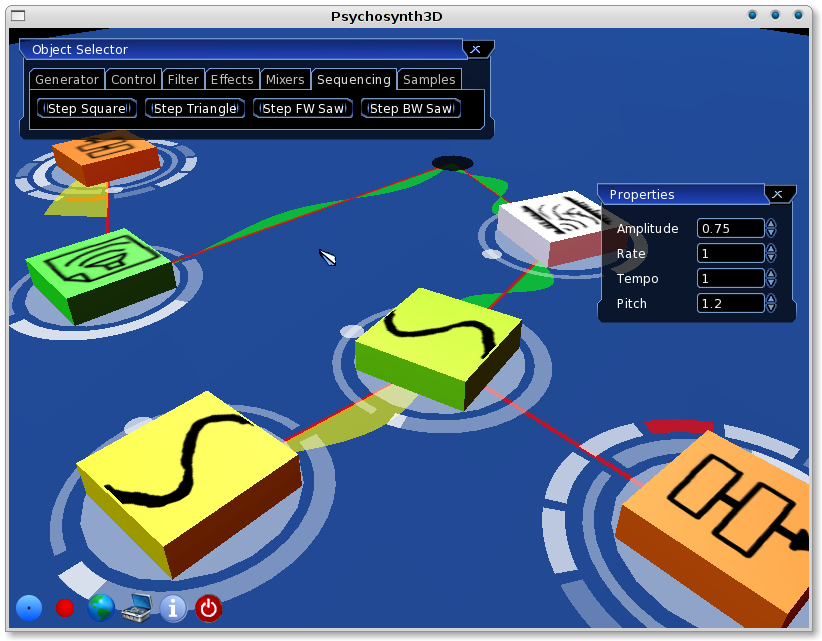
\includegraphics[width=\textwidth]{pic/screenie.png}
  \caption[A screenshot of GNU Psychosynth 0.1.4]{A screenshot of GNU
    Psychosynth 0.1.4.}
  \label{fig:screenie}
\end{figure}

\subsection{A critique on the term framework}

The term \emph{framework}\index{framework} is used many times in this
and other projects and is becoming a techie buzzword. In many contexts
it is abused as a synonym for the term
\emph{library}\index{library}. Instead, we believe that a framework is
something different, following the definition given in the famous
design patterns book by the gang of four \cite{gamma95design}.

We use the term \emph{library} when the root of the call graph is on
the client side and the client invokes the library functions to obtain
some concrete functionality. Instead, a \emph{framework} stands in the
root of the call graph and the client code is called through extension
hooks in the framework, following the ``Hollywood
principle''\index{Hollywood principle} --- ``Don't call us, we'll call
you.''.

Because the Psychosynth system is layered, one can just use the bottom
layers as a library, or rely on the upper layers that properly use
inversion of control\index{inversion of control} like a framework.

\subsection{The layered architecture}

At the current stage, GNU Psychosynth implements a layered
architecture\index{layered arquitecture} \cite{garlan94software}. This
tries to achieve a more decoupled design, as calls between modules are
only allowed from top down.

Also, the library has many features, many of which some users may not
need. This layered approach could allow a potential user to avoid any
special overhead when she is only using some bottom layers. Still,
note that the library is currently compiled will all layers bundled in
the same shared-object file, so this is not an advantage yet. Because
the heavy redesign ongoing during this project, we shall postpone that
until later development stages when layer interactions are clear and
stable.

Figure \ref{fig:layers} represents the current layered
architecture. The vertical arrows represent function calls. The big
arrow that crosses through all layers represents the fact that all
layers are allowed to use the facilities of the \emph{base}
layer. Thus, a layer is allowed to use the facilities in the layer
below and the \emph{base} layer only --- e.g. the \emph{graph} layer
uses the \type{synth} and \type{base} API's in its
implementation. Lets make a bit more in-depth discussion of each
layer.

\begin{figure}[h!]\centering
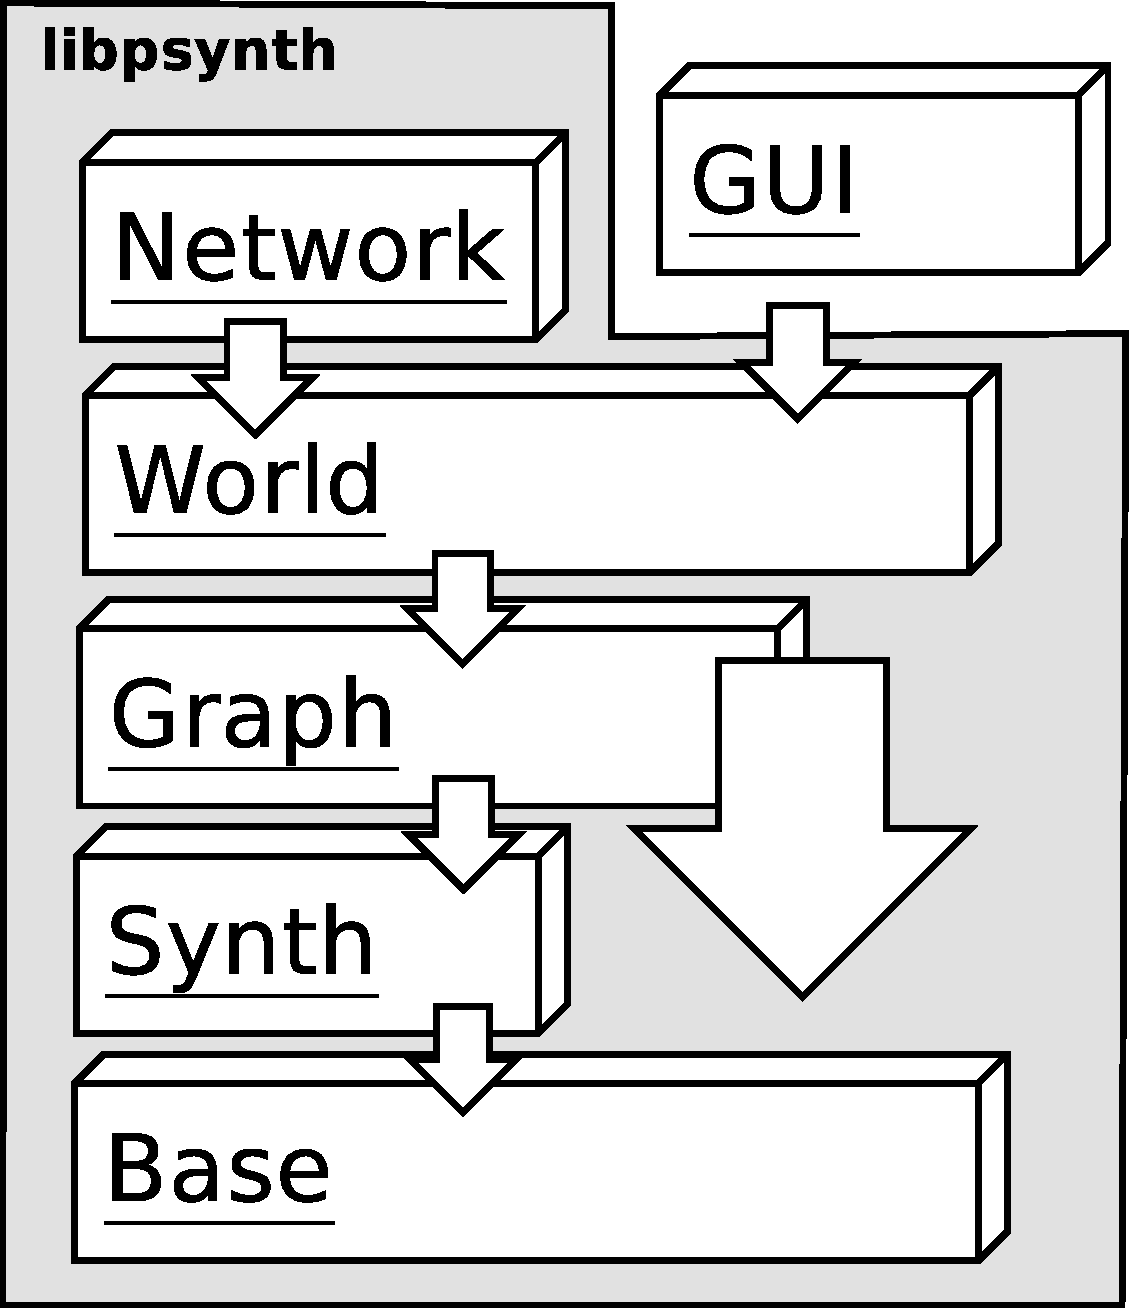
\includegraphics[width=.6\textwidth]{pic/layers.pdf}
\caption{The GNU Psychosynth layered architecture.}
\label{fig:layers}
\end{figure}

\subsubsection{The \texttt{base} layer}

The base layer\index{base (layer)} includes basic facilities that may
be reusable in any other part of the application. Some of the most
relevant examples are:

\begin{description}
\item[Configuration persistence] Classes for representing program
  settings in a hierarchical manner. This configuration system can use
  interchangeable backends and has an observable
  interface.\footnote{We use quite often the term \emph{observable
      interface} which is rare in the literature. By this, we mean
    that it provides signals, listeners or other event mechanisms,
    instances of the \emph{observer} design
    pattern\cite{gamma95design}.}

  In fact, we do not recommend using this module in the core of the
  intermediate layers of the library because it can cause unexpected
  coupling. Maybe in the future it will be moved to the thin
  \emph{app} module, but it is kept here for historical reasons.

\item[Implementation of design patterns] While the term \emph{design
    pattern}\index{design pattern} means reusable design structure,
  not reusable code, language abstractions can make them implementable
  generically in some cases. Andrei Alexandrescu proves this point for
  C++ in \cite{alexandrescu01modern}. This layer provides design
  pattern generic implementations inspired by Alexandrescu's
  approach. Some of the included facilities are implement
  \emph{observer}, \emph{singleton} and \emph{composite}.

\item[Command line argument parsing]\index{command line arguments}
  While we have considered moving to Boost's Program Options
  library\footnote{\url{http://www.boost.org/doc/libs/release/doc/html/program_options.html}},
  our own implementation have different trade-offs and is rather
  extensible.

\item[Logging system]\index{logging} A hierarchical and multi backend
  logging system for registering messages from other modules. It
  should be used instead of direct output to \texttt{std::cout/cerr}
  in all the code.

\item[File management tools] That ease the task of finding resources
  in the hard-drive and can cache results.
\end{description}

Some other minor classes and tools are excluded from this list. During
the development of the project we will drop in this layer classes that
feel interesting at any abstraction level.

\subsubsection{The \texttt{synth} layer}

\index{synth (layer)}This layer contains classes for the \emph{static}
construction of synthesisers and sound processing. The audio input and
output facilities are considered to be in this layer, and as well
audio processing data structures,--- like ring buffers, multi channel
buffersm, etc. --- basic implementations of filters, oscillators and
audio scalers.

By static, we mean that this code does not provide any dynamic routing
facilities, instead, the programmer is in charge to assign buffers and
call the processing elements manually.

Requisites \ref{req:iter1-begin} to \ref{req:iter1-end} should be
implemented here. Non functional requisites \ref{req:iter1-begin2} to
\ref{req:iter1-end2} are specially relevant in this layer too. Indeed,
this layer should be divided in three parts: the sound representation
library, the IO classes and the synthesis algorithms.

\subsubsection{The \texttt{graph} layer}

\begin{figure}[h]
\centering
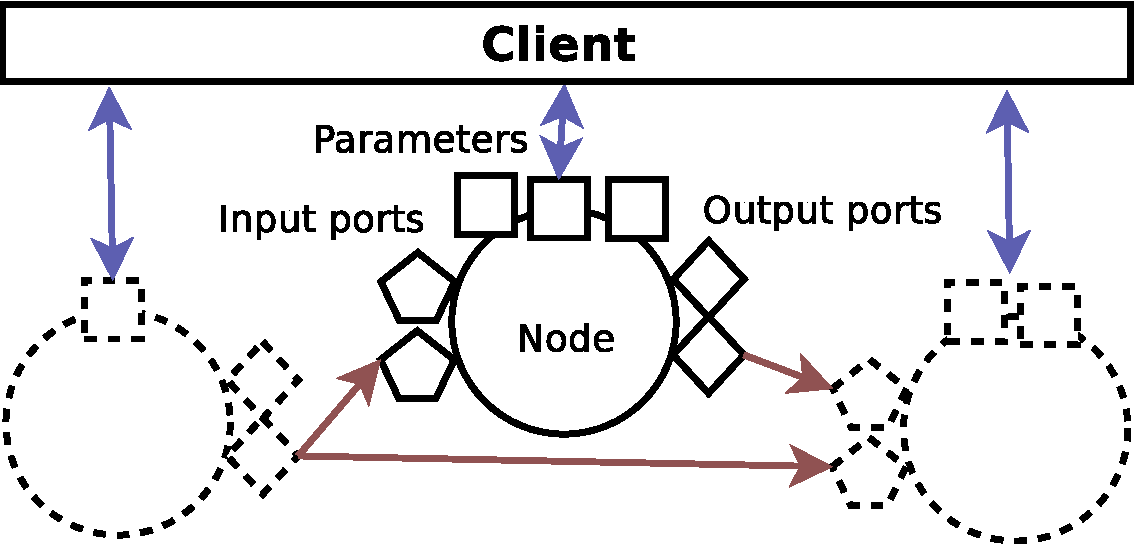
\includegraphics[width=.8\textwidth]{pic/node.pdf}
\caption[Representation of the node graph as in Psychosynth
0.1.7]{Representation of the node graph as in Psychosynth 0.1.7. Input
ports are represented as pentagons, output ports as rombus and
parameters as squares.}
\label{fig:node}
\end{figure}

This layer provides the facilities for the \emph{dynamic} construction
of synthesisers. It includes the mechanisms for describing and
executing the modular synthesis graph with the signal flow and so
on. Figure \ref{fig:node} represents the main concepts behind the
current design. Ports are considered as ``signal ports'' using the
terminology in requirement \ref{req:porttype} --- ``control ports''
are similar to ``parameters'', but parameters are not a precise model
of ``control ports'' as they can not be routed and are intended for
communication between the client user interface code and the audio
thread state. The communication system used to propagate values
between the audio processing thread and the client thread is
represented in figure \ref{fig:thread}. Values are copied to and from
an intermediate channel between the audio processing blocks.


\begin{figure}[h]
\centering
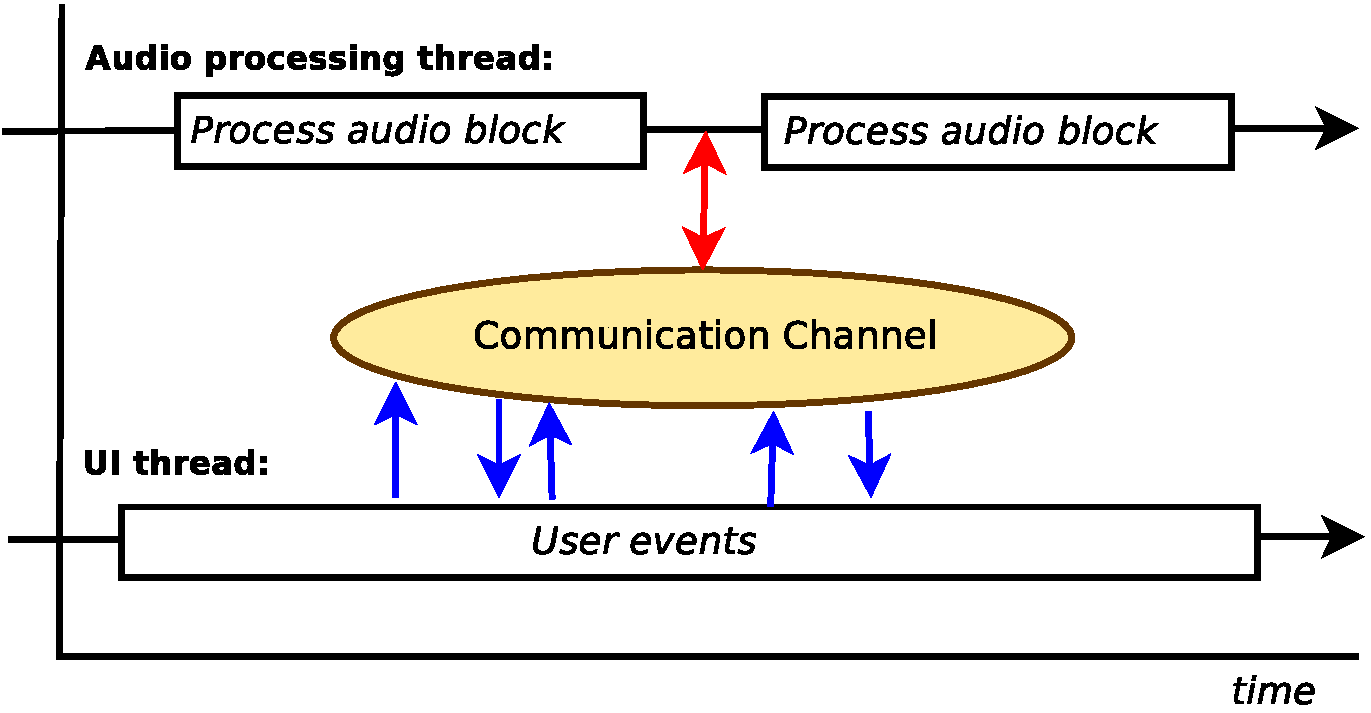
\includegraphics[width=.8\textwidth]{pic/thread.pdf}
\caption{Communication between the audio and user interface thread as
  in Psychosynth 0.1.7}
\label{fig:thread}
\end{figure}

Requisites \ref{req:iter2-begin} to \ref{req:iter2-end} should be
implemented in this layer. A heavy redesign of its API and many of its
internal implementation is to be expected for that to be
accomplished.

\subsubsection{The \texttt{world} layer and the Model View Controller
  architecture}

This layer simplifies the interface exposed to the previous layer and
makes it \emph{observable}\index{observer (design pattern)}. This is
fundamental for the Model View Controller that the system implements.
Figure \ref{fig:mvc} represents this architectural style. On the
following, we can refer to this observable interface abstracting the
synthesis engine as \emph{the model}\index{model (MVC)}.

\begin{figure}[h!] \centering
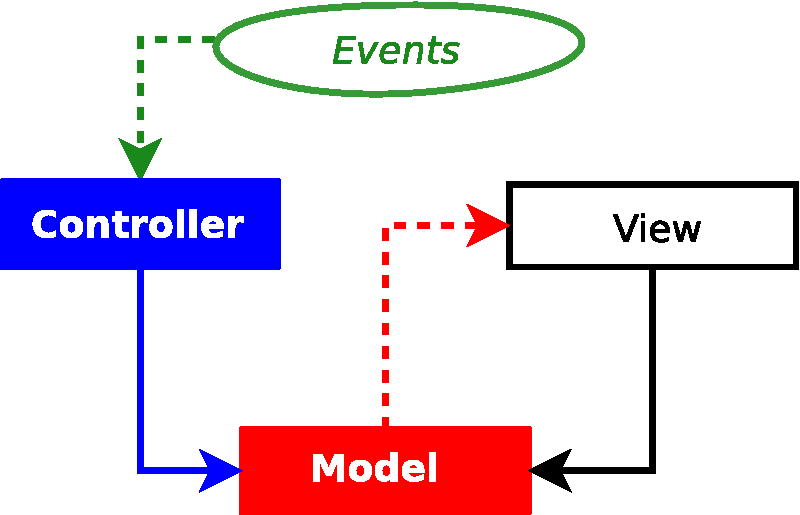
\includegraphics[width=.7\textwidth]{pic/mvc.pdf}

\caption[The MVC architectural style]{The Model View Controller
  arquitectural style. Dashed arrows represent indirect invocation
  ---i.e. via the \emph{observer} design pattern--- and normal lines
  represent normal method calls and data access.}
\label{fig:mvc}
\end{figure}

Several views\index{view (MVC)} can coexist independently --- for
example, a GUI user interface and a web client ---, that get updated
whenever a value has changed in the model. They register themselves on
the model at the beginning and then become passive entities that get
called by the model. The model changes when controllers invokes
methods on it, several controllers\index{controller (MVC)} can
coexists too. Usually, models and views come in pairs. For example, a
GUI view has an associated controller that triggers the manipulation
of the model in the eventuality of certain user actions like clicking
a button; in this case the representation (the buttons) and the action
(clicking it) are strongly related, but this is not necessarily true
in other situations.

This layer also abstracts the graph interconnection mechanism using
the \emph{strategy} design pattern\index{strategy (design
  pattern)}. Concretely, dynamic patching is implemented here and the
interface exposed in this layer hides the manual node interconnection
mechanisms but provides observability for topological changes.

This layer should implement requisite \ref{req:views}. 

\subsubsection{The application framework layer and some built-in views
  and controllers}

There is a thin layer, instance of the \emph{facade}
pattern\index{facade (design pattern)}, called \texttt{app}. It was
hidden for simiplicity in figure \ref{fig:layers} representing the
layered architecture. It sits on top of the \texttt{world} layer and
is in charge of initialising the \emph{world}, defines a configuration
tree using the facilities in the \texttt{base} layer, and setups the
machinery using the observability of the configuration system to keep
coherence between the user preferences and the status of the synthesis
model --- for example, if the ``\texttt{psynth.output}'' setting is
changed, it automatically creates the appropriate output object
instance, sets its values and substitutes the output node in the
synthesis graph. This layer also sets up the command line argument
parsing and installs some common audio setting arguments in the
parser. This layer is where Psychosynth becomes a
framework\index{framework} at its most pure level, as it offers a
\texttt{psynth\_app} class whose \texttt{run} method should be the
only call in the program \texttt{main}. This in turn delegates the
heavy work to user code that is hooked as method overrides of that
same class.

Orthogonal to this layer, and also sitting on top of the
\texttt{world} layer, the networking\index{networking} layer offers a
set of views and controllers\footnote{A primitive implementation of
  such at this stage of the development.}  that can be used to create
the shared environment described in requirement \ref{req:sharedenv}
--- thus enabling collaborative performances. This is an example of
the value of the MVC architecture: because views and controllers are
orthogonal, the user interface does not need to know about the
presence of this component to function properly. One could develop a
new experimental and cool UI and it would automagically be optionally
able to work with third party clients over the network, even
potentially using a different user interface.

In its current version, on top of all this, there is the code of the
3D user interface and some small and simple command line tools
intended to be used as GUI-less network capable clients and
servers. But all this code is not part of the framework. Instead, the
framework remain user interface agnostic, so we will not further
describe the UI code as it falls outside the scope of this project.

\section{Project planning and methodology}

\subsection{Rationale --- A critique on software engineering}

\index{software engeneering}Choosing a well known software engineering
process is considered one of the first steps to be taken in a final
master's thesis project. In our school we study with most detail the
Waterfall Model\index{waterfall model} \cite{benington87production}
and the Rational Unified Process\index{RUP, rational unified process}
\cite{kruchten03rup}.

Those development processes propose a fordist software production
model, targeted at huge development teams and the development of
stable code bases in non-experimental, well defined, fields. Many of
their proponents state that software engineering is like any other
engineering where creative analysis and design is only the first step
--- thus they believe programming is analogous to construction.
Fowler makes a great point \cite{fowler01design} criticising this
argument, as he says, the construction is done by the compiler and
people involved in programming are actually doing an intellectual and
creative work too --- in computing, any systematic task can and must
be automated indeed. The $programming=construction$ metaphor is
alienating for the programmer, who is completely excluded from the
task of criticising and improving the software design, and thus this
metaphor often leads, in the end, to bad software.

Moreover, these fordist development models take risk control and
client requirements satisfaction as most important factors. Because we
are in an academic environment, there are two more important factors:
the pedagogical value of the project --- this is, that the student
involved takes the risk of exploring the unknown by himself --- and
the research value --- this is, that the student involved takes the
risk of exploring the unknown by humanity.

Of course, this is neither a pure research project, so we can not
completely substitute a software development process by the scientific
method. But we can choose a more dynamic methodology that includes
\emph{falsification} in one way or the other. \emph{Agile}
methodologies\footnote{\url{http://agilemanifesto.org/}} propose many
alternatives that could be valid for a master thesis project.

Still, these methodologies are, we believe, inadequate for this
concrete project. The main reason is that this project is developed by
only one person. Agile methodologies put most emphasis on the
developer communication methods and collective decision making, so
they are often inadequate and too constraining and time consuming for
an unipersonal team, providing no additional value.  The Personal
Software Proccess \cite{watts96psp} proposes a methodology that is
specially targeted at personal software developed by engineering
students. Sadly, we are not very familiar with it --- and do not have
enough time to make that happen within the time constraints of the
project --- and it seems too be to specific and time consuming in its
time tracking proposal.

Because we still believe that some rational planning and methodology
is needed, we propose in the following a defined but unconstrained
methodology that is specially tailored for our circumstances,
capturing the most common elements in other software processes.

\subsection{An iterative development model}

Because of the size and complexity of the project, we should not
consider developing it all at once. Moreover, the layered architecture
of the starting code base and the variety of requirements that we want
to satisfy favour an iterative development.

Consequently, we want to split the development in iterations. Each
iteration is composed by the following phases: \emph{design},
\emph{implementation}, \emph{verification} and
\emph{integration}. Each iteration shall be assigned a set of
requirements from the specification in section \ref{sec:requirements}
that are to be satisfied after the successful accomplishment of that
iteration.

\subsubsection{The design phase}

\index{design}In the design phase we shall define the API that we
would like the current subsystem to have. Because we are developing a
library and framework with a public interface, the design phase is
specially relevant shall be done with care.

We do not enforce a particular method for documenting the design as
different programming paradigms favour different documentation
means. For example, in the first iteration we will develop a library
heavily based on metaprogramming, where UML does not fit very
naturally. Still, the documentation should include rationale
explaining why the design decision lead to the satisfaction of the
requirements assigned to that iteration. Also, it may be found that a
requirement may be impossible to satisfy on the current iteration or
that this requirement is to be better integrated in some other
iteration. The developer is free to reassign that requisite for later
iteration properly documenting this as a post-analysis plan fix.

What we do enforce is that all the API is documented with Doxygen for
the sake of completeness of the reference manual.

\subsubsection{The implementation phase}

\index{implementation}During the implementation phase the code
implementing the design should be written. It is possible and even
sometimes recommended to modify the design during this phase as
inconsistencies and fundamental problems are found. Sometimes, this
may even start as soon as design, specially when it is unclear the
properties that such API should have and some ``exploratory
programming'' is needed. This fact may or many not be documented in
the design document --- even though an API may be designed through an
inductive empirical process, a deductive rational description may be
more useful for its clear understanding indeed.

We are keen on Test Driven Development\index{TDD, test driven
  development} \cite{beck02tdd}. This methodology suggests that unit
tests should be written before the actual implementation for the
tested interface is written at all. Instead, a mock implementation is
to be provided. Once the tests compile --- and fail --- implementation
is started concentrating on making the tests pass. Once the tests do
pass, the code and internal design is improved via
\emph{refactoring}\index{refactoring}. We will not follow this
methodology dogmatically --- specially when exploratory programming is
required --- but we suggest to follow it whenever possible. Thus, we
can consider than the verification phase and implementation phase are,
or at least should be, overlapped.

\subsubsection{The verification phase}

\index{verification}In the verification phase we perform \emph{unit
  tests} on the most important parts of the system. No iteration
should be considered finished unless proper unit tests are written and
satisfied for its core components. For writing such tests the Boost
Unit Testing Framework should be used.

When some elements are considered relevant to performance
requirements, \emph{performance tests} should be included. While we do
not enforce a specific performance testing technique here, the
tests should be reproducible and automatable whenever possible.

\subsubsection{The integration phase}

\index{integration}When a subsystem is added and it is to replace an
existing subsystem in the project, the older code should be removed
and the layers on top must be modified such that they use the new
code. This might even be sometimes considered part of the
verification, as older tests working on the upper layers should be
checked to be working after the integration.

Informal integration tests should be done on the final user interface
to make sure that the properties of the older implementation are
preserved. Note that in most cases, we do not recommend to lose time
editing the old user interface such that the new features in the
framework are exposed to the user. Of course, that the new features
are usable is the final objective, but as it was justified in
\ref{sec:userinterface}, a completely new user interface will be
developed as part of a future project.

\subsubsection{Recursive decomposition of iterations}

In practice, some of the expected requirements to be satisfied may be
found orthogonal or maybe too big to be addressed at one. It is thus
allowed to recursively decompose an iteration in sub-iterations when a
first evaluation during the design phase suggests that.

\subsection{A project plan}

In the following we propose a project plan to accomplish the
requirements specified at the beginning of this chapter. As we stated
in the introductory chapter, this is a long-term project, and the
required effort to fulfil all the proposed objectives clearly exceeds
what a student can do in parallel to his normal studies\footnote{The
  student involved in this project, apart from being studying the
  normal courses for the 5th year in ``Ingeniería Informática'', he is
  also collaborating with the Computer Vision Group in the development
  of Moodle plug-ins (\url{http://nongnu.org/cvg-moodle/}), and has
  been hired by the Institute of Astrophysics of Andalucia to held a
  course in Advanced Python Programming in May
  (\url{http://sinusoid.es/python-avanzado/}). These time constraints
  must be taken into account in the project planning.}. \emph{Thus,
  only the two first iterations are to be developed in this mater's
  thesis}. This structure fits very well in the Spanish university
course structure; the first iteration shall be developed during the
first semester and the second iteration during the second and last
semester.

\subsubsection{First iteration: A metaprogramming based sound
  processing foundational library}

\begin{description}
\item[Description] In this iteration involves a deeply re-design the
  core data structures using the latest techniques in C++. This
  requires special research. Performance requirements deeply rely on
  the success of this iteration.

\item[Criterion] Requirements \ref{req:iter1-begin} to
  \ref{req:iter1-end} and \ref{req:iter1-begin2} to
  \ref{req:iter1-end2} should be satisfied for its success.

\item[Estimated time cost:] 4 months.
\end{description}

\subsubsection{Second iteration: Redesign of the \texttt{node} layer}

\begin{description}
\item[Description] The \texttt{node} layer requires a redesign if we
  want it to scale to satisfy all our long-term purposes. Polyphony
  and hierarchy would be specially tricky to implement directly on top
  of the current code base. A special evaluation of how the new design
  interacts with the MVC architecture and networking is required. The
  \texttt{world} layer may be affected too. The whole layer should be
  reimplemented and validated.

\item[Criterion] Requirements \ref{req:iter2-begin} to
  \ref{req:iter2-end} should be satisfied for its success. Requirement
  \ref{req:persistence} may be optionally considered for its
  implementation in this iteration too.

  \item[Estimated time cost] Estimated time cost: 4 months.
\end{description}

\subsubsection{Third iteration: Dynamic loading of nodes}

\begin{description}
\item[Description] In this iteration the plugin system is to be
  developed. This involves loading of nodes with our own interface ---
  as designed in the previous iteration --- and with external
  interfaces, implementing interface adaptors when needed.

\item[Criterion] Requirements \ref{req:iter3-begin} to
  \ref{req:iter3-end} should be satisfied for its success.

\item[Estimated time cost] 3 months.
\end{description}
\subsubsection{Fourth iteration: Adding MIDI and synchronisation}

\begin{description}
\item[Description] Synchronisation and MIDI support is one of the most
  important features and it is also one of the features we know the
  least about, thus, we should put special care on research and
  design. This will affect the node and world layers mostly.

\item[Criterion] Requirements \ref{req:iter4-begin} to
  \ref{req:iter4-end} should be satisfied for its success. Requirement
  \ref{req:polyphony} might be implemented in this iteration too.

\item[Estimated time cost] 5 months.
\end{description}

\subsubsection{Post mortem analysis}

After the conclusion of all the previous iterations, we should write a
conclusive report and evaluation of the project's success. Also, we
should prepare a final presentation for the project evaluation.

\begin{mynote}[Structure of the rest of the documment]
  The rest of the documment is devoted for documenting the modules
  developed in the iterations that are expected to be developed within
  this master's thesis. Chapter \ref{sec:03-meta} describes the first
  iteration involving the new sound system. Chapter \ref{sec:04-graph}
  explains the new graph layer as developed in the second
  iteration. Finally, chapter \ref{sec:05-conclusion} recapitulates
  and will provide some sort of post-mortem analysis --- of these two
  iterations --- also preparing the ground for the future development
  of the project.
\end{mynote}

%%% Local Variables: 
%%% mode: latex
%%% TeX-master: "00-main"
%%% End: 
